\documentclass[11pt,a4paper]{article}

\usepackage{mynotes}

\title{A regional scale assessment of the biodiversity - ecosystem function relationship in southern African woodlands}
\author{John L. Godlee}
\date{}

\begin{document}

\maketitle
\tableofcontents

\section{Introduction}

A number of studies have shown relationships between biodiversity and ecosystem functionality \citep{Review}. The strength and direction of these observed relationships varies depending on the ecosystem being studied \citep{}, the ecosystem function(s) of interest \citep{}, and the inclusion of environmental covariates in statistical models \citep{}, but there appears to be a generalisable positive correlation between biodiversity and ecosystem functionality \citep{Liang2016}. Over the past decade, many observational studies of the Biodiversity-Ecosystem Function Relationship (BEFR) have been conducted in tropical and temperate forests, and grasslands \citep{Chen2011}. The representation of dry tropical ecosystems in the BEFR literature however, is poor. \citet{Clarke2017} conducted a meta-analysis of 182 published BEFR studies, finding that only 13\% were conducted in the tropics, with 42\% of those being conducted in the highly endemic wet tropical forests Costa Rica.

In the seasonally dry woodlands of southern Africa, human actions are driving rapid changes in biodiversity. Resource extraction directly influences biodiversity via selective tree-felling for timber, charcoal making, non-timber forest products and through land use change to agriculture \citep{Ryan2016}. Climate change is also indirectly affecting the biodiversity of southern African woodlands, altering temperature and precipitation, and affecting climate seasonality \citep{}. Savannas and sparse woodlands are the dominant vegetation type across the southern African region, spanning \textgreater{}4 million km\textsuperscript{2}. The carbon stored in these woodlands is comparable to that found in the wet forests of the Congo basin and are of global importance to the carbon cycle. Climatic conditions and biogeography vary across southern African woodlands, resulting in a diverse range of woodland tree species assemblages, which retain the common features of an open tree canopy and an understorey generally dominated by C4 grass species \citep{Frost1996}. Southern African woodlands are highly diverse, thought to harbour \textapprox{}8500 plant species of which there are \textgreater{}300 tree species \citep{Frost1996}. These ecosystems have been identified by previous studies as a priority for conservation efforts \citep{Brooks2006, Mittermeier2003, Frost1996}. Many conservation projects in the region currently aim to conserve biodiversity and woody biomass stocks simultaneously under the banner of REDD+ \citep{Hinsley2015}. A small number of academic studies in these woodlands have shown that above ground woody carbon/biomass stocks correlate positively with tree species richness \citep{McNicol2017, and, others}, but all have been hampered by a restricted climatic and biogeographical range of study sites, meaning that generalisable regional trends cannot be reliably inferred. \citet{Fayolle2018} 

The role of environmental factors in mediating the BEFR generally is poorly understood \citep{Ratcliffe2017}. Climatic variation is known to affect woody biomass \citep{Michaletz2014}, so it is important to account for these factors and acknowledge their interaction with both woody species diversity \textit{and} biomass stocks to effectively model the effects of biodiversity on biomass stocks in a regional analysis. \citet{Sankaran2005} used data from 854 African woodland field sites to show that mean annual precipitation sets the upper limit for woody cover in these ecosystems, which is presumably positively correlated with biomass \citep{}, while other factors such as herbivory, fire regime and soil properties also contribute at a local scale to reduce woody cover below this maximum. However, this study did not consider the role of species diversity in the complex interactions between environment and tree cover. 

\citet{Condit2013} found that dry season intensity was the main determinant of tree species distribution in Panamanian tropical forests, which may affect ecosystem level productivity and thus woody biomass through selection effects, promoting the growth of a certain highly productive species only under specific environmental conditions. In European forests \citep{Ratcliffe2017} found a general trend towards stronger positive relationships between tree species richness and various ecosystem functions in more arid environments, suggesting variation in the balance between competitive and facilitative effects along the aridity gradient as the driver of this relationship, an example of the Stress Gradient Hypothesis \citep{Dohn2013}. Water availability imposes a physiological limit on growth rate, which interacts with mortality due to stochastic processes such as fire and herbivory to limit maximum potential woody biomass \citep{}. 

Temperature imposes a similar physiological limit on woody growth rate by limiting metabolic rates. Temperature and water availability together impact the transpiration rate of a tree, with high temperatures and low water availability limiting growth and potentially causing damage or mortality through cavitation of vessels within the tree \citep{Rowland2015a, Fensham2009}. In southern African woodlands however, many species are drought adapted and lose their leaves in the dry season, limiting water loss \citep{Solbrig1996}, so this effect may not be present in historically droughted areas. The effect of extreme climatic conditions on woody biomass may depend on the degree to which the current biota is adapted to it. Furthermore, across many forested ecosystems, water availability, modulated through precipitation and soil type positively correlates with tree species richness \citep{Vila2005}, meaning that extremely arid areas may be limited in their potential ecosystem functionality via two effects, the direct effect of resource availability in the form of moisture availability and soil nutrients, and indirectly through the effect of these environmental factors on species composition. Species composition may therefore have a greater effect on the interaction between environment and biodiversity - ecosystem function relationships, than species richness \textit{per se}.

\todo{Species abundance evenness and selection effects.}

While southern African woodlands are species rich in the herbaceous understorey, the tree layer is relatively species poor \citep{}. \citet{Miombo-Book} however, writes that they are structurally diverse in the tree layer, with trees of the same species occupying distinct layers of the canopy at different growth stages. This structural diversity may be one mechanism through which species diversity appears to influence woody biomass. Trees occupying different canopy layers can create a more full canopy with a greater total foliage density, enhancing productivity and allowing greater standing woody biomass in a smaller area. An underpinning principle of the Biodiversity-Ecosystem Function Relationship (BEFR) is that of niche complementarity. Species are assumed to differ in their functional niche by the fact that they may coexist in a steady-state ecological community, therefore the more species are present the greater the area of the total fundamental niche of the ecosystem is filled, allowing more efficient use of natural resources and higher gross primary productivity and biomass \citep{}. This theory however, which has been supported by many experiments and observational studies in temperate and wet tropical ecosystems, may not hold in savannas, which are structured by disturbance rather than competition.

High levels of disturbance in the form of seasonal fires and herbivory from large mammals \citep{Fire is a herbivore} may moderate the strength of observable BEFRs in southern African woodlands. Fire disturbance in forests has been linked to abundance dependent mortality among smaller stems \citep{Roques2001}. A dominant and competitive species which tends to produce many small fast-growing stems is more likely to experience mortality during a fire as the higher surface area to volume ratio of the trunk increases the likelihood of combustion \citep{}. Such fast-growing bushy species exist in southern African woodlands and often proliferate when fire is deliberately excluded, leading to the growth of thicket vegetation which precludes the growth of high biomass tree species \citep{nieto2018}. Additionally, the dominance of a single species is likely to decrease overall functioning by decreasing niche space utilisation \citep{Cardinale2002}.

In this study, we made the first known regional estimation of the Biodiversity-Ecosystem Function Relationship in southern African woodlands, using inventory plots which straddle multi-dimensional environmental and biogeographical gradients (Figure \ref{}). We used aboveground woody biomass \todo{and estimates of ecosystem productivity} as measures of ecosystem functionality to understand the co-relationship between tree species biodiversity and ecosystem functionality. We compared the relative effects of tree species biodiversity with that of other environmental factors known to affect ecosystem productivity and biomass accumulation such as precipitation and temperature. In acknowledgement of the wide variation in biogeographically determined community composition across the region, we also used biogeographical clusters \citep{} to understand how species composition as well as species biodiversity \textit{per se} affected ecosystem functionality. Initially, we made four hypotheses: 1) across the region, after other environmental factors had been accounted for, woodland plots with a higher species richness would have a higher aboveground biomass, 2) increased aridity would increase the strength of the biomass tree species richness relationship, 3) species composition would have a greater affect on aboveground biomass than species diversity \textit{per se}. We used Structural Equation Modelling as a preferred method to simultaneously account for environmental factors and biogeographic factors, which often interact in their effect on ecosystem structure and therefore biomass. 


\subsection{Hypotheses}

\begin{enumerate}
	\item{Plots with a higher tree species diversity will maintain higher biomass stocks.}
	\item{Species abundance evenness will influence above-ground productivity more than species richness \textit{per se}.}
	\item{Plots in more arid regions will feature a stronger positive effect of tree species richness on above ground biomass stocks, due to abiotic facilitation effects, despite lower overall tree species richness.}
	\item{Structural characteristics of the woodland will interact with species composition and richness to provide an indirect path of influence between species composition and biomass stocks.}
\end{enumerate}


\section{Methods}

\subsection{Study location}

The study used 1066 woodland monitoring from a larger network located across 10 countries within southern Africa in so-called Miombo woodland (Figure \ref{plot_loc}). The study region spans a precipitation gradient from \textapprox{}460 mm y\textsuperscript{-1} in the \todo{where} and \textapprox{}1700 mm y\textsuperscript{-1} in the \todo{where}. The study sites straddle the climate space of the region as a whole (Figure \ref{temp_precip_hull}a). The 2D convex hull of Mean Annual Precipitation (MAP) and Mean Annual Temperature of the study sites covers 92.7\% of the pixel-wise climate space of the Miombo woodland area as defined by \citet{White}, using WorldClim estimates of temperature and precipitation between the year 1970 and 2000 with a pixel size of 30 seconds (0.86 km\textsuperscript{2} at the equator). 

\begin{figure}[H]
	\centering
	\subfloat[]{{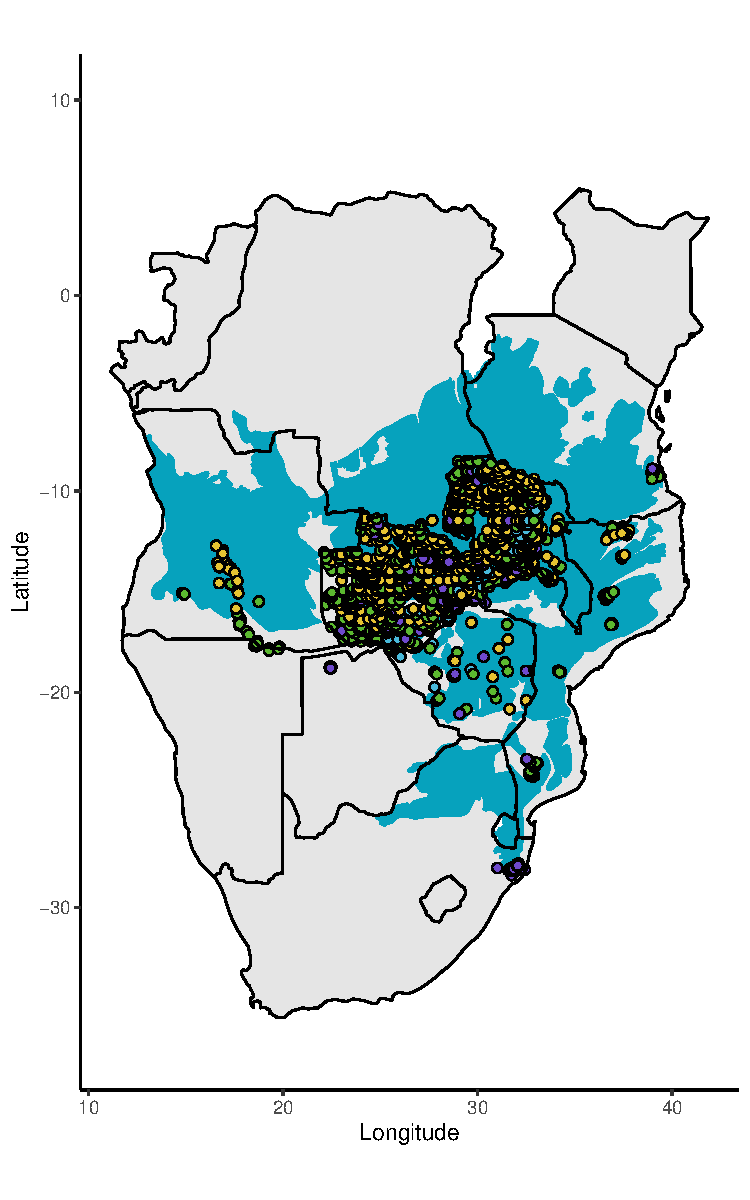
\includegraphics[width=0.4\textwidth]{plot_loc}}}%
    \qquad
    \subfloat[]{{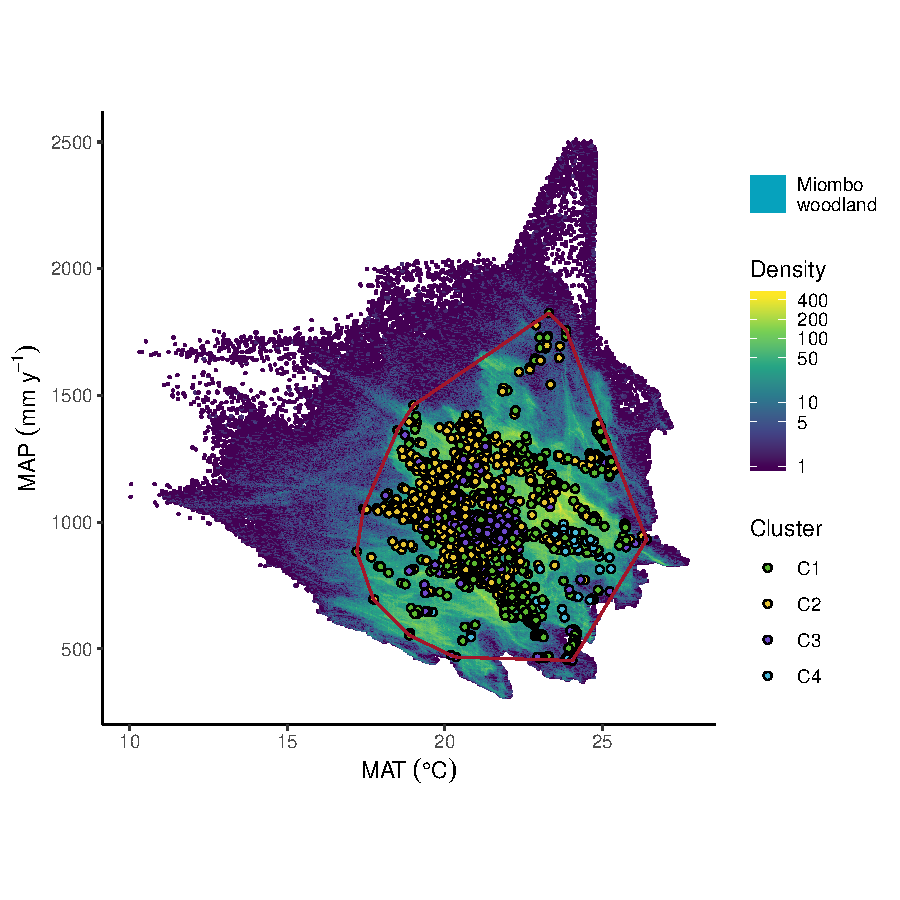
\includegraphics[width=0.4\textwidth]{temp_precip_hull}}}%
    \caption{The locations of the 1066 plots used in this study, by geographic location (a) with respect to the distribution of Miombo woodland vegetation \citep{White}, and in climate space (b), showing the plot locations as points compared to the climate space of the whole region as estimated using the WorldClim dataset over the Miombo woodland vegetation extent.}
\end{figure}

Plots were chosen from a larger pool of 5395 plots based on the quality of data collection and plot setup. Plot vegetation was identified under the broad term of ``savanna'', which includes ``woodland'', ``savanna woodland'', and ``tree savanna''. Plots with evidence of farming, human resource extraction or experimental treatements such as prescribed burning or herbivore exclusion were exlcuded from the initial pool. Only plots \textgreater{}0.1 hectares were used as per hectare biomass estimation from small plots is highly influenced by rare large trees. Only plots with a stem density \textless{}10 stems ha\textsuperscript{-1} were used, to ensure all plots were within woodland rather than ``grassy savanna'', which are considered a separate biome with very different species composition \citep{Parr2014}.

Many plots provided by the Zambian Forestry Commission were arranged in clusters of four 20x50 m plots, 20 metres apart. These plots were aggregated for analyses and their values averaged for use in further plot level data cleaning.

A Principle Coordinate Analysis (PCoA) was conducted on tree species abundance matrix data for each plot to identify compositional outliers, which were considered not representative southern African woodlands. Plots within the upper 95th percentile of plot neighbour distance in the PCoA were excluded from further analyses (Figure \ref{pcoa_outlier}). This removed 66 plots.

\begin{figure}[H]
\centering
	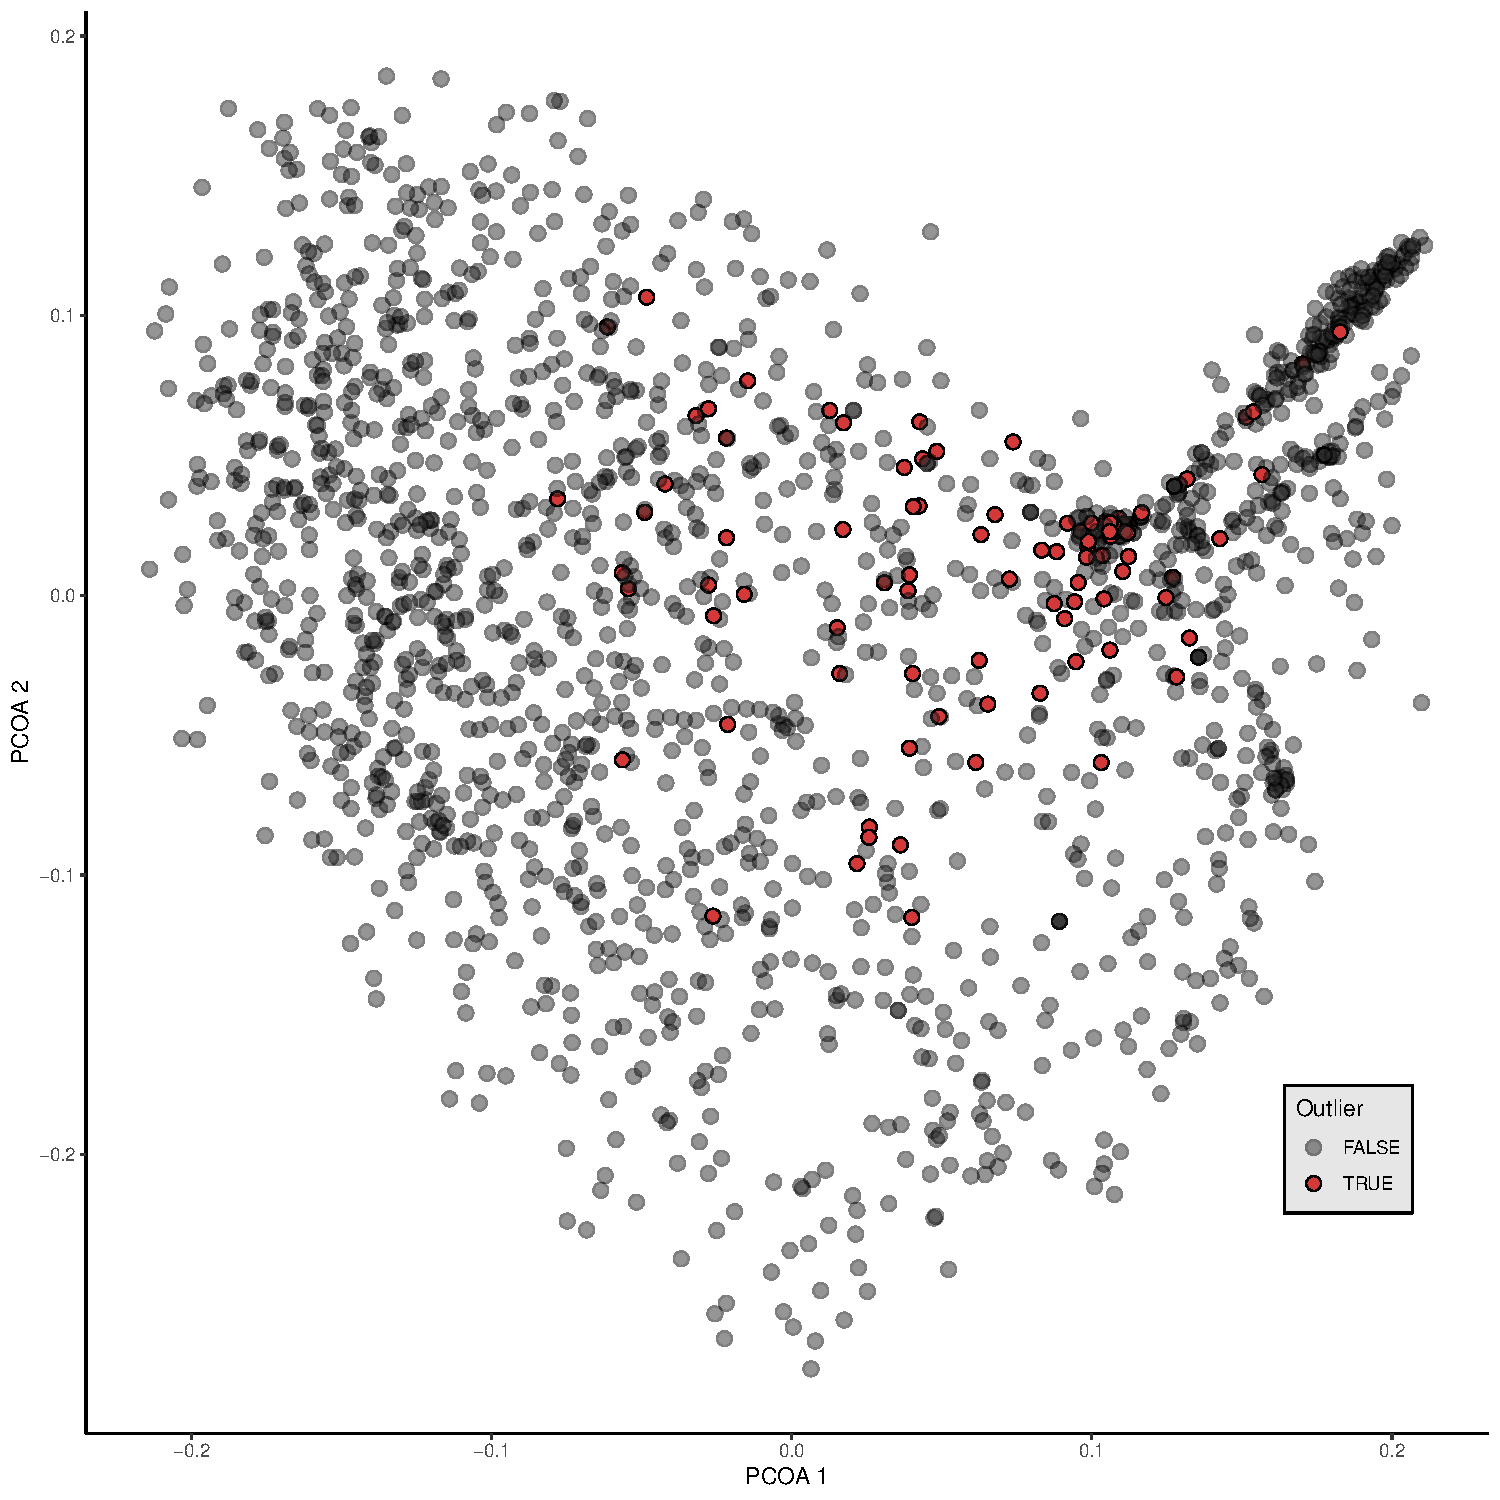
\includegraphics[width=0.5\textwidth]{pcoa_outlier}
	\caption{Principle Co-ordinate Analysis of tree species diversity of the 1122 plots chosen from the larger pool of 5395 plots. The PCoA is constructed from a tree species abundance matrix. Plots which are within the upper 95th percentile of plot neighbour euclidean distance in the PCoA are marked in red, to be excluded from further analysis.}
	\label{pcoa_outlier}
\end{figure}

\subsection{Data collection}

We considered only trees and shrubs in our analyses of above-ground biomass, including woody species including palms and cycads but excluding lianas. Only stems \textgreater{}5 cm DBH (Diameter at Breast Height, 1.3 m) were included in analyses. AGB estimation for trees \textless{}5 cm DBH is imprecise due to its sensitivity to many environmental and historical factors \citep{}. Additionally, for some species, species identification is difficult for saplings.

All stems \textgreater{}5 cm DBH were measured within each plot. For each tree, species, DBH and height to the highest branch material were recorded. Height was measured through a variety of means including laser rangefinders, manual clinometers and measuring sticks, which resulted in a variety of measurement uncertainty in the dataset, however, averaged over such a large number of stems this should not meaningfully alter the results of our analysis. When DBH could not be measured at 1.3 m due to trunk abnormalities, it was measured at the closest regular portion of the trunk to 1.3 m. The height of this measurement was recorded and used to estimate the DBH\textsubscript{e} at 1.3 m using a cubic polynomial, parameters estimated using a test dataset \citep{Ryanunbublished}.

Aboveground biomass for each plot was calculated using Equation \ref{chave_agb}, taken from \citet{Chave2014}. Wood density estimates were taken from the global wood density database for each species where possible \citep{Chave2009, Zanne2009}. Wood density for species without species level estimates was estimated from the mean of their respective genus. 

\begin{equation}
	AGB_{est} = 0.0673 \times (\rho D^{2} H)^{0.976}
	\label{chave_agb}
\end{equation}

Where $\rho$ is the species level mean wood density, $D$ is the DBH at 1.3 m, and $H$ is the tree height.

Climatic data was collected from the ECMWF ERA5 dataset \citep{}. Values were aggregated for each year between 2000 and 2018, then averaged across the years to provide single values per plot. Temperature and precipitation seasonality were both calculated as the coefficient of variation of these variables across the 18 years of available data. Soils data was extracted from the \todo{WHERE}. 

Fire return interval ($F_{ret}$) was calculated using the MODIS burned area product V6 (MCD46A1) \citep{}. Data was downloaded from January 2000 to December 2018. Mean fire return interval was calculated as:

\begin{equation}
	F_{ret} = \frac{\sum_{i = 1}^{n} t_{i} - t_{i-1}}{n-1}
\end{equation}

Where $t_{i}$ is the date of fire $i$, and $n$ is the total number of fires in the time period. Fire return interval data was binned into five ordinal categories ranging from ``frequent fire'' to ``no fire''. Bin values for categories where fire had occurred were defined as four bins with percentiles based on equal numbers of plots. Plots without a single fire recorded in the 18 year survey period were assumed to not be affected by fire. 

\subsection{Data analysis}
Rarefied species richness accounted for variation in plot size and therefore sampling effort across the region. Rarefied species richness was calculated using the \verb|vegan| package in R, using a sample size of 20 stems. Plot size varied from 0.1 hectares to 10 hectares.

To assess tree species abundance evenness, the Shannon Equitability index \citep{} (Equation \ref{shannon_equit}) was calculated: 

\begin{equation}
	E_{H'} = \frac{-\sum_{i = 1}^{s} p_i \ln{p_i}}{\ln{S}}
	\label{shannon_equit}
\end{equation}

Where $p$ is the proportion abundance of a tree species $i$ across all individuals in the plot and $S$ is the total number of species in the plot.. The numerator of the Shannon Equitability index ($E_{H'}$) is the frequently used Shannon-Wiener diversity index ($H'$).


\subsubsection{Biogeographical clusters}

Plots were assigned to biogeographical groups, after \citet{Fayolle2018}. Groups were identified in \citet{Fayolle2018} using an Africa wide analysis of floristic units using plot data in savannas with tree species diversity and relative abundance data. Groups were identified using unconstrained correspondence analysis and ordination. Plot data used in this study occurred in five biogeographical groups, see Table \ref{clust_tabl} for a description of each biogeographical cluster.


\subsubsection{Structural Equation Modelling}

Structural Equation Models (SEM) investigated the regional determinants of woody Above-Ground Biomass (AGB). All SEMs were constructed and analysed in the \textit{lavaan} package in R version 3.6.0. SEM was used because of its suitability for modelling complex causal interactions in ecological systems \citep{Lehmann2014_161-166}. A key aspect to our decision to use SEMs is that they can explicitly model indirect effects, which is impossible in multiple regression. Using SEMs also allowed us to describe theoretical latent constructs which have been suggested by theory to act upon diversity and biomass/productivity in previous studies despite these factors not having single observable values in our dataset. For example, moisture availability is known to affect productivity, but it's actual value is determined by the interaction of multiple observable variables over the time scales relevant to tree lifetime growth: precipitation, the seasonality of that precipitation, and soil composition. Indepedently of total precipitation, precipitation seasonality (measured as the covariance of daily precipitation) determines, simplistically, whether water arrives uniformly over a given time period or as few high volume floods, the latter leading to much water being lost before it can be used for plant growth. 

We specified a conceptual model with latent variables based on theoretical unmeasured factors known to affect AGB: moisture availability, temperature suitability for plant growth, soil fertility, fire regime intensity, tree species diversity and tree structural diversity (Figure \ref{con_mod}). Although the fire regime composite only had a single indicator variable, it was nevertheless included in a latent variable to soak up measurement error \citep{}.

\begin{figure}[H]
\centering
	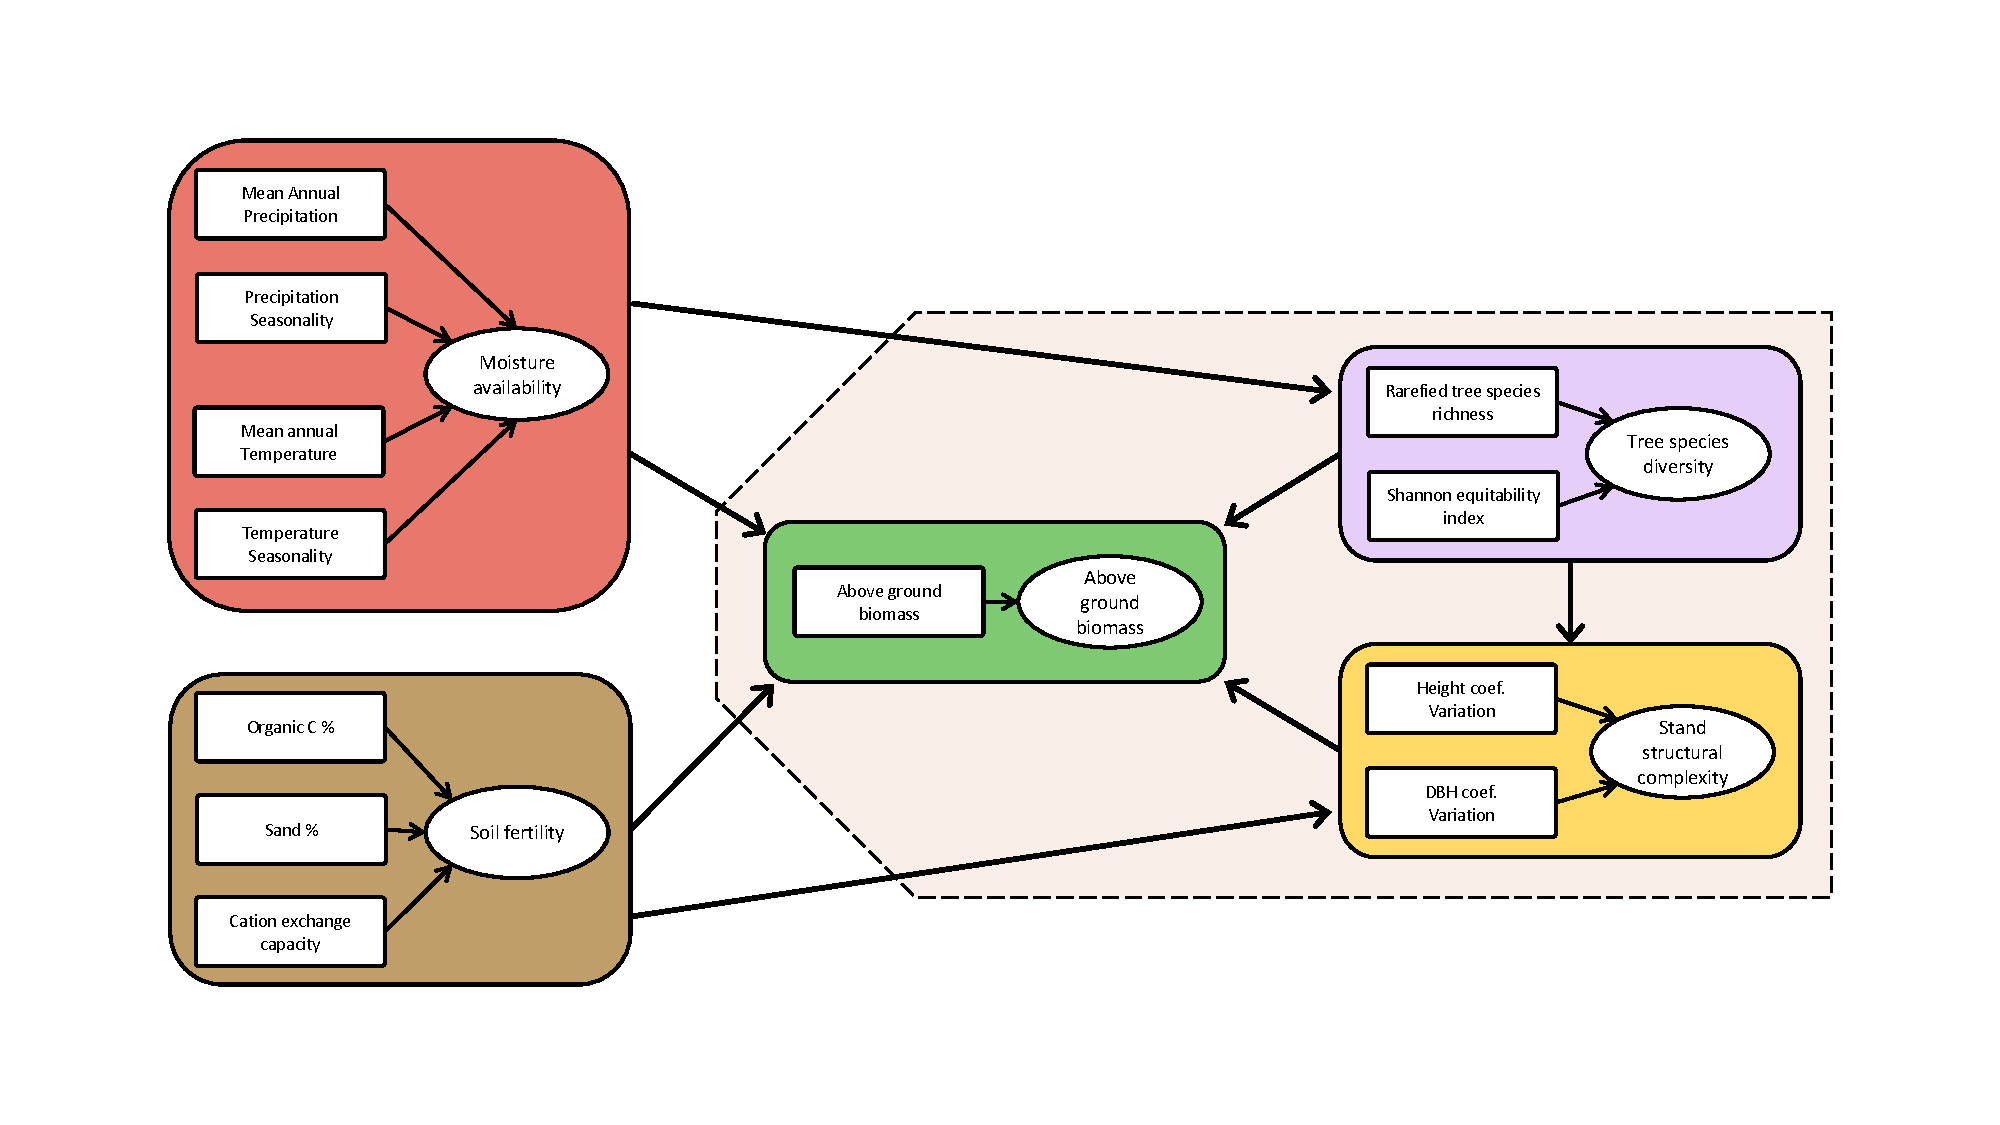
\includegraphics[width=0.8\textwidth]{con_mod}
	\caption{Conceptual model showing the theoretical relationships between environmental factors, structural and species tree diversity and AGB. Hypothesised paths of causal inference are depicted as arrows from predictor to response.}
	\label{con_mod}
\end{figure}

Observed variables of the latent variables were standardized to Z-scores for analysis. Standardization put each latent variable on the same scale, with a mean of zero and a standard deviation of one. It allows path regression coefficients to be easily compared between paths to assess their relative effect strength, and eliminates problems arising from the observed variables being on different scales. Standardization also controls for variables with different orders of magnitude which could otherwise prevent adequate model estimation from the covariance matrix.

The factor loadings of the observed variable assumed to contribute most to each latent variable were set to 1 as per convention \citep{}. Due to some latent variables being regressed against both structural diversity and AGB, exact factor loadings from multiple regressions against either of these response variables could not be used to inform factor loadings in the SEM and were therefore estimated by the SEM model.

For each biogeographical cluster, and at the regional level, we employed SEM to assess the relative importance of each latent variable in determining AGB. We assessed the indirect effects of abiotic environment on AGB via species and structural tree diversity to understand the interactive nature of species diversity and abiotic environment in determining AGB. In a model selection process, latent variable paths for each biogeographical cluster model were removed sequentially to investigate their removal on model fit. Model fit at each stage of the model selection process was evaluated using the Comparative Fit Index (CFI), the Tucker Lewis Index (TLI) and the R\textsuperscript{2} coefficient of determination for AGB. The best models according to these goodness-of-fit statistics are presented in the results. See \todo{Appendix 1 for a full description of all models in the model description process.}

Two sets of SEMs were fitted. The first used only tree diversity latent constructs to estimate diversity, with the indirect effect of species diversity on AGB via structural diversity being explicitly modelled as a mediation effect to examine the strength and form of this relationship. The second incorporated environmental covariates to understand the relative effects of climate, soils, disturbance on diversity and AGB.

\section{Results}

\begin{figure}[H]
\centering
	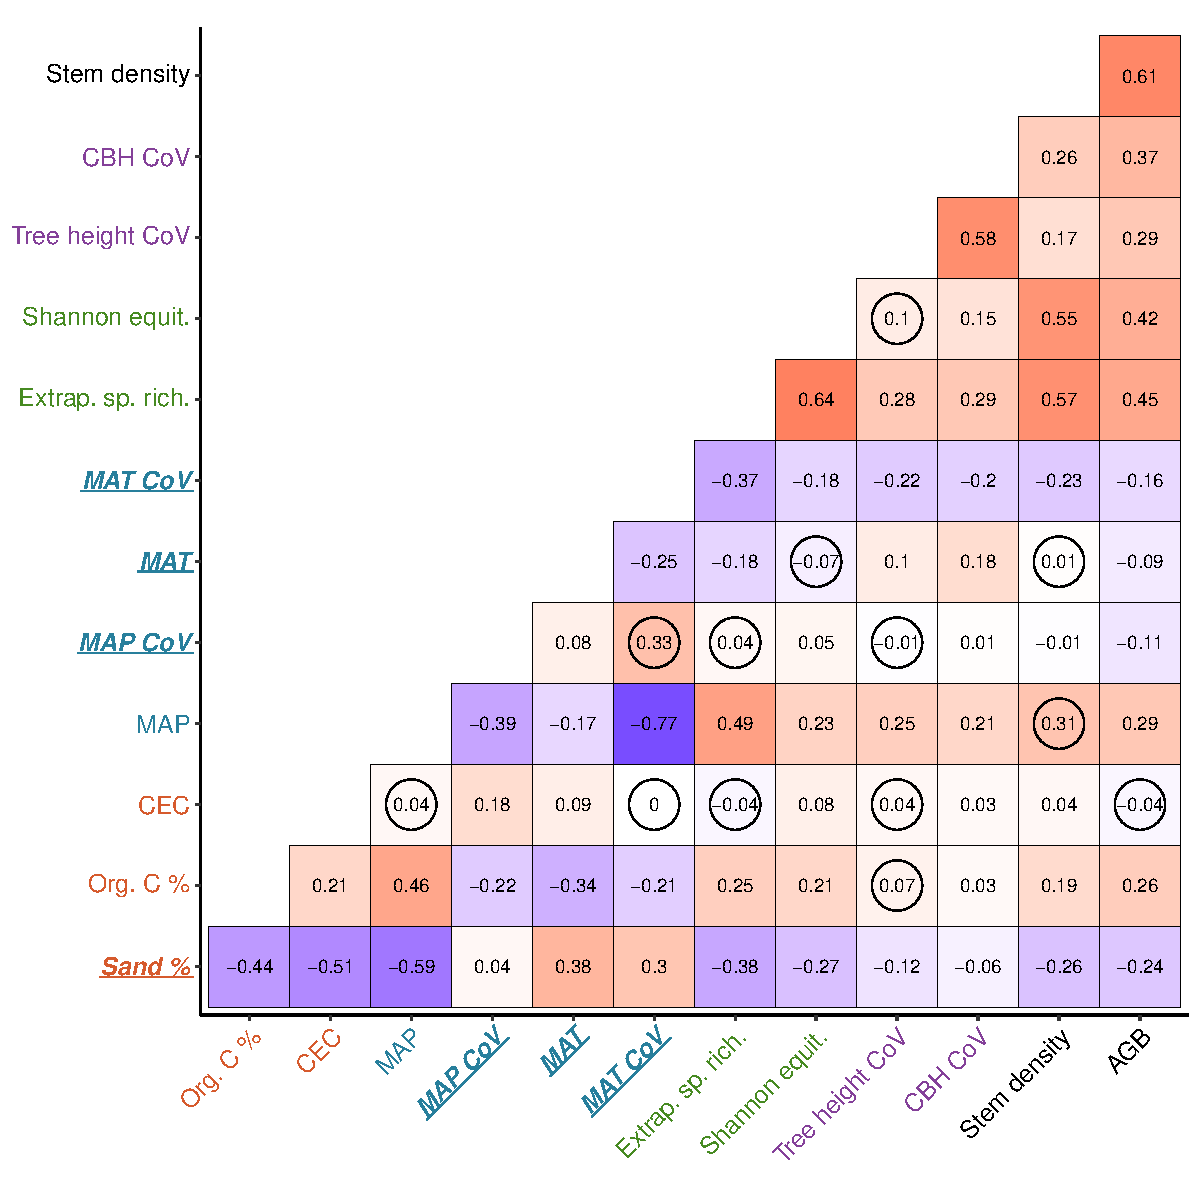
\includegraphics[width=0.6\textwidth]{corr_mat}
	\caption{Correlogram of exogenous variables used in the analysis, with correlation coefficients shaded according to sign (+ve red, -ve blue) and strength of correlation.}
	\label{corr_mat}
\end{figure}

Simple correlations showed a positive association between Aboveground Biomass (AGB) and a latent variable representing tree species diversity ($r_{(1522)}$ = 0.30, $t$ = 12.2). The tree structural diversity latent variable also had a positive association with AGB ($r_{(1327)}$ = 0.18, $t$ = 15.0).

In an SEM describing the indirect effect of tree species diversity on AGB via the mediating effect of stand structural diversity, species diversity had a negative effect on AGB when the indirect path via stand structural diversity was accounted for (Figure \ref{struc_model_slopes}). Stand structural diversity had a strong positive effect on AGB (\todo{Test stats}). This effect was observed in biogeographical clusters 1, 2 and 3. Clusters 4 and 5 had small sample sizes due to missing data and so path regression uncertainties were high, with confidence intervals overlapping zero. 

\begin{figure}[H]
\centering
	\includegraphics[width=\textwidth]{struc_model_slopes_clust_all}
	\caption{Path coefficients (slopes) for the effects of tree diversity on AGB, mediated by the effect of stand structural diversity. Path coefficients are +/- 1 standard error. Path coefficients where the standard error does not overlap zero are considered to be non-significant effects.}
	\label{struc_model_slopes}
\end{figure}


% Table created by stargazer v.5.2.2 by Marek Hlavac, Harvard University. E-mail: hlavac at fas.harvard.edu
% Date and time: Fri, Jan 17, 2020 - 12:26:16
\begin{table}[!htbp] \centering 
  \caption{} 
  \label{struc_model_fit_clust_stats} 
\begin{tabular}{@{\extracolsep{5pt}} ccccccccc} 
\\[-1.8ex]\hline 
\hline \\[-1.8ex] 
cluster & ntotal & chisq & df & cfi & tli & logl & rmsea & rsquare\_agb \\ 
\hline \\[-1.8ex] 
Marginal miombo & $525$ & $44.750$ & $6$ & $0.966$ & $0.916$ & $$-$3714.000$ & $0.110$ & $0.710$ \\ 
Core miombo & $668$ & $57.210$ & $6$ & $0.962$ & $0.904$ & $$-$4224.000$ & $0.100$ & $0.680$ \\ 
Baikiaea & $47$ & $5.860$ & $6$ & $0.998$ & $0.994$ & $$-$324.600$ & $0.030$ & $0.720$ \\ 
Mopane & $84$ & $9.420$ & $6$ & $0.971$ & $0.927$ & $$-$591.600$ & $0.080$ & $0.450$ \\ 
All & $1324$ & $78.430$ & $6$ & $0.975$ & $0.936$ & $$-$9119.000$ & $0.090$ & $0.690$ \\ 
\hline \\[-1.8ex] 
\end{tabular} 
\end{table} 


\begin{figure}[H]
\centering
	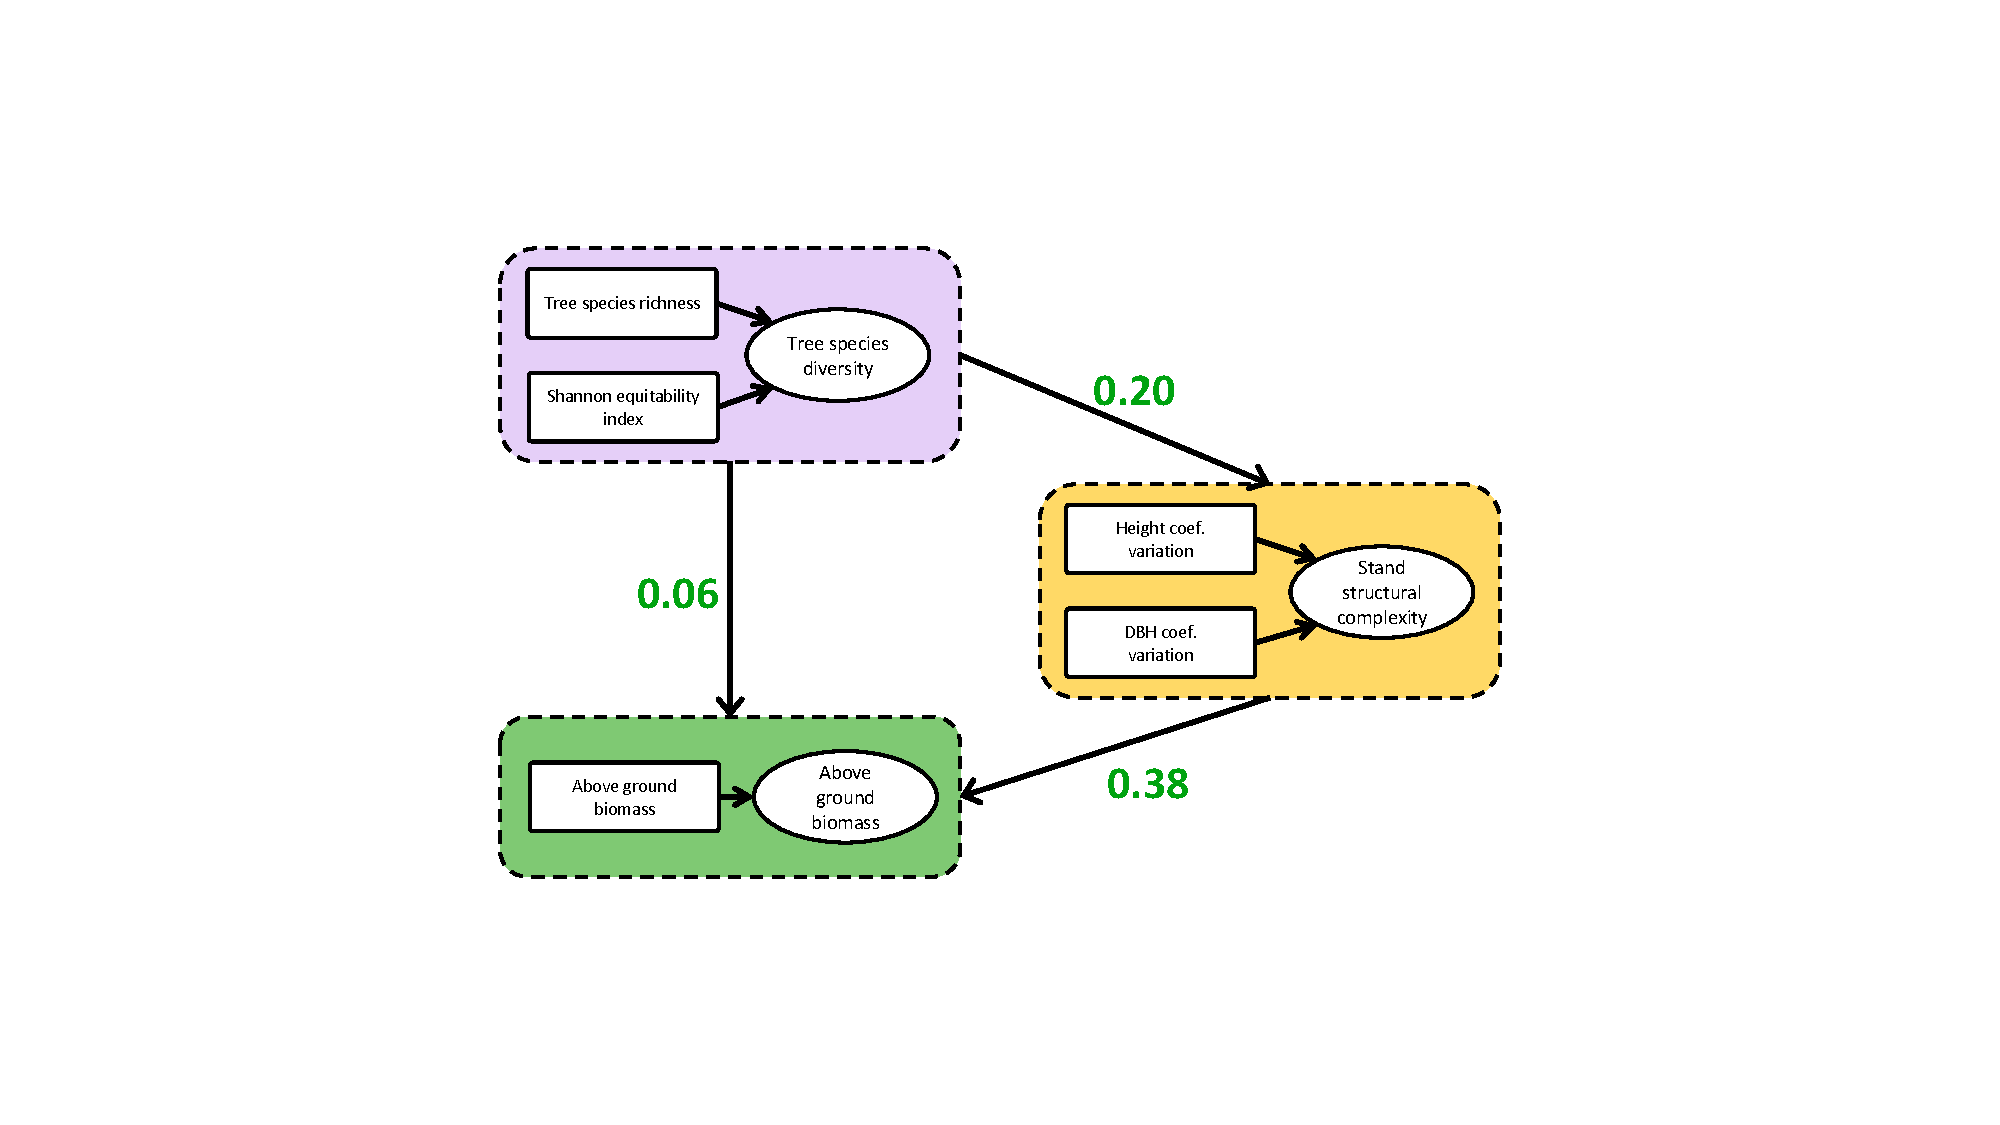
\includegraphics[width=\textwidth]{sem_struc_path}
	\caption{Path diagram with regression coefficients for the structural model including plots in all five clusters.}
	\label{sem_struc_path}
\end{figure}

\begin{figure}[H]
\centering
	\includegraphics[width=\textwidth]{full_latent_model_slopes}
	\caption{Path coefficients (slopes) for the interactive effects of abiotic environment and tree diversity on AGB across all plots. Path coefficients are +/- 1 standard error. Path coefficients where the standard error does not overlap zero are considered to be non-significant effects.}
	\label{full_latent_model_slopes}
\end{figure}

\subsection{Structural diversity}

The latent variable of tree species diversity had a weak positive effect on AGB across the region. A stronger positive effect was seen between structural diversity and aboveground biomass, with species diversity acting \textit{through} structural diversity to effect aboveground biomass.

\section{Discussion}

%\bibliography{/Users/johngodlee/google_drive/bib/lib}


\end{document}

% Seidel 2019: Large trees tend to possess a greater structural complexity than small trees, not due to their size per se, but due to more complex architecture.
